We performed a K Nearest Neighbor for $K\in[0,150]$ to see how it performed.
% \begin{figure}
%     \centering
%     \includegraphics[width=0.5\linewidth]{}
%     \caption{Caption}
%     \label{fig:enter-label}
% \end{figure}
As seen in figure \ref{fig:KNN} KNN performs best at $K=6$ with an accuracy of 84.2\%, which is not our best performing model, but slightly better than the most naive classifier.

\begin{figure}[h!]
    \centering
    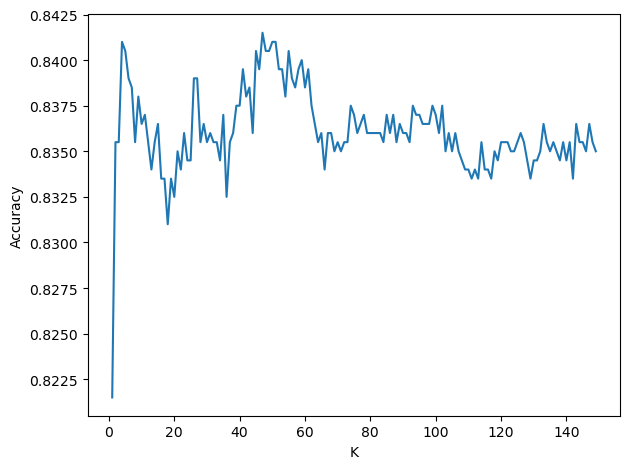
\includegraphics[width=0.8\columnwidth]{Plots/KNN_150accuracy.png}
    \caption{Box plots of sample data}
    \label{fig:KNN}
\end{figure}